\documentclass[dvipdfmx]{report} % 文章の形式を設定
\usepackage[margin=2.5cm]{geometry} % 書式の空白を設定
\usepackage[utf8]{inputenc} % 文字コードをUTF-8に設定
\usepackage{hyperref} % 目次にリンクを付けるため
\usepackage{lipsum} % ダミーテキスト用
\usepackage{tcolorbox} % 枠を利用するため
\usepackage{amsmath} % 数式の記述を行うため
\usepackage{bm} % ベクトルを太字で表示するため
\usepackage{graphicx} % 画像を表示するため
\usepackage{float} % 画像正しい位置で表示するため
\usepackage{tensor} % テンソルを記載するため
\usepackage{multicol} % 複数段落を作成するため
\usepackage{tikz} % 図を作成するため

\title{勉強したこと(雑記)}
\author{大豆生田 幹}
\date{}

\begin{document}

\maketitle % タイトルの作成
\tableofcontents % 目次の作成

\chapter{2024 05/15}
% =================================
% chapter 1
% =================================

\section{特殊相対論}

% 特殊相対論の復習
\subsection{ガリレイ変換}
ある慣性系$O$と、その系と比較して$x$軸方向に$V(m/s)$で進む慣性系$O'$を考える。\\
すると、$O$での座標$(x, y, z)$と$O'$での座標$(x', y', z')$の関係は以下のようになる。\\
\begin{eqnarray}
    x' = x - Vt \\
    y' = y \\
    z' = z
\end{eqnarray}
このような変換をガリレイ変換という。\\
この変換は、運動方程式
$$F_x = m\ddot{x}$$
を不変にする。

\subsection{ローレンツ変換}
時刻$t_0$で$(x_1,y_1,z_1)$を出発する光は\\
時刻$t_1$で$(x_2,y_2,z_2)$に到達する。\\
このことから、
$$( c(t_1-t_0) )^2 = (x_1-x_0)^2 + (y_1-y_0)^2 + (z_1-z_0)^2$$
が成り立つ。\\
どの慣性系においても光速度$c$が一定であれば、この等式は常に成り立つはずである。\\
そこで、この量を$s_{12}$と置き、世界間隔と呼ぶ。\\
$$s_{12} = (x_1-x_0)^2 + (y_1-y_0)^2 + (z_1-z_0)^2 - (c(t_1-t_0))^2$$
\\
座標が$(t,x,y,z)$で表される系をミンコフスキー時空と呼び、\\
この系の変換で世界間隔を不変にするものをローレンツ変換という。\\
\\
ある慣性系$O$と、その系と比較して$x$軸方向に$V(m/s)$で進む慣性系$O'$を考える。\\
すると、$O$での座標$(t, x, y, z)$と$O'$での座標$(t', x', y', z')$の関係は以下のようになる。\\
\begin{eqnarray}
    x' = \frac{x - Vt}{\sqrt{1 - \frac{V^2}{c^2}}} \\
    y' = y \\
    z' = z \\
    t' = \frac{t - \frac{Vx}{c^2}}{\sqrt{1 - \frac{V^2}{c^2}}}
\end{eqnarray}
このような変換をローレンツ変換という。\\
以下の式を計算すれば、ローレンツ変換が世界間隔を不変にしていることがわかる。
$$
    (c(t_1-t_0))^2 - (x_1-x_0)^2 =
        c^2 \Biggl{(}\frac{t_1- \frac{Vx_1}{c^2}}{\sqrt{1-\frac{V^2}{c^2}}} - \frac{t_0- \frac{Vx_0}{c^2}}{\sqrt{1-\frac{V^2}{c^2}}} \Biggr{)} ^2 -
        \Biggl{(}\frac{x_1 - Vt_1}{\sqrt{1-\frac{V^2}{c^2}}}-\frac{x_0 - Vt_0}{\sqrt{1-\frac{V^2}{c^2}}} \Biggr{)}^2
$$

\section{
    オイラーラグランジュ方程式の導出
}
システムの数学的なモデルを「作用」と呼び、これを具体的に考える。\\
作用は関数を入力すると実数を返すような関数になっており、汎関数という。\\
力学の原理は「作用が最小となる運動が実現する」というものである。\\
$$S[q]=\int^{b}_{a}{L\bigl{(}q(t),\dot{q}(t)\bigr{)}dt}$$
この定積分はいつ最も小さく条件を探す。\\
\\
ある関数形$q$で$S[q]$が最小となるとき、$q$の形を少し変形したとしても$S$の値はほとんど変化しないことに注目する。\\
十分に小さい量(2次以上を無視できる)$\epsilon$、任意の関数$f(t)$を用いて、$q$から無限小だけ変形した関数$\tilde{q}$を考える。\\
$$
\tilde{q}(t)=q(t)+\epsilon f(t)
$$
この時、$f(t)$は$a < f < b$以外で$0$とする。\\
$S[\tilde q]-S[q]$の値を考えると
$$
S[\tilde q]- S[q] = \int^{b}_{a}
{ L \bigl{(}\tilde q(t), \dot{\tilde q}(t)\bigr{)} - L\bigl{(}q(t), \dot{q}(t)\bigr{)}dt}
$$
$$
= \int^{b}_{a}
{ \bigl{(} L\bigl{(}q(t)+\epsilon f(t), \dot{q}(t)+\epsilon \dot{f}(t)\bigr{)} - L\bigl{(}q(t), \dot{q}(t)\bigr{)} \bigr{)}dt}
$$

ここで、2変数関数のテイラー展開を思い出す
\begin{tcolorbox}[title=2変数関数のテイラー展開]
    2変数関数$F(x,y)$について、$(a,b)$周りでのテイラー展開は以下のようになる。
    $$
    F(x,y) = F(a,b) + \frac{\partial F}{\partial x}|_{x=a}(x-a) + \frac{\partial F}{\partial y}|_{y=b}(y-b) +
    $$
    $$
    \frac{1}{2!}\frac{\partial^2 F}{\partial x^2}|_{x=a}(x-a)^2 + \frac{\partial^2 F}{\partial x \partial y}|_{x=a,y=b}(x-a)(y-b) + \frac{1}{2!}\frac{\partial^2 F}{\partial y^2}|_{y=b}(y-b)^2 + \cdots
    $$
\end{tcolorbox}
これを使い、$\epsilon$の2乗以上の項を無視すると、
$$
S[\tilde q]- S[q] = \int^{b}_{a}
{ \bigl{(} \frac{\partial L}{\partial q}\epsilon f +  \frac{\partial L}{\partial \dot{q}}\epsilon \dot{f} \bigr{)} dt }
$$
これを部分積分すると
$$
= \epsilon \int_{a}^{b}{ \bigl{(} \frac{\partial L}{\partial q} - \frac{d}{dt} (\frac{\partial L}{\partial \dot{q}}) \bigr{)} f dt} + 
\epsilon \int_{a}^{b}{ \frac{d}{dt} \bigl{(} \frac{\partial L}{\partial \dot{q}} f \bigr{)} dt}
$$
$a < f < b$以外で$0$としていたことを思い出すと、
$$
\frac{\partial L}{\partial q} - \frac{d}{dt} (\frac{\partial L}{\partial \dot{q}}) = 0
$$

\section{
    エネルギー保存則の導出
}
$p_i = \frac{\partial L}{\partial \dot{q_i}}$として、\\
エネルギーを
$$
E = \sum_{i=1}^{n}{p_i \dot{q_i} - L}
$$
と定義する。\\
これが時間に依存しないことを示す。\\
$E$を時間で微分すると、
$$
\frac{dE}{dt} =
\sum_{i=1}^{n}
{\bigl{(} \dot{p_i} \dot{q_i} + p_i \ddot{q_i} \bigr{)} } -
\biggl{(}
\sum_{i=1}^{n}{ \frac{\partial{L}}{\partial{q_i}} \dot{q_i} } +
\sum_{i=1}^{n}{ \frac{\partial{L}}{\partial{\dot{q_i}}} \ddot{q_i} } + 
\frac{\partial{L}}{\partial{t}}
\biggr{)}
$$
$$
= \sum_{i=1}^{n}{\biggl{(}
\dot{q_i}\bigl{(} \dot{p_i} - \frac{\partial{L}}{\partial{q_i}} \bigr{)} +
\ddot{q_i}\bigl{(} p_i - \frac{\partial{L}}{\partial{\dot{q_i}}} \bigr{)} -
\frac{\partial{L}}{\partial{t}}
\biggr{)}}
$$
ここで、オイラーラグランジュ方程式
$$
\dot{p_i} = \frac{\partial{L}}{\partial{q_i}}
$$
より、
$$
\dot{E} = - \frac{\partial{L}}{\partial{t}}
$$
つまり、エネルギーが保存することは、ラグラジアンの形が時間に依存しないことによる。


\chapter{2024 05/22}
% =================================
% chapter 2
% =================================

\section{
    特殊相対論
}
\subsection{
    アインシュタイン収縮
}
静止した慣性系$O$で静止したペンの長さを世界間隔で測る。\\
ここで、簡単のため座標は$(ct, x)$のみを考える。\\
ペンの片端を$(0, 0)$と置くと、もう片端の位置が$(0, L)$となっている。\\
この時、世界間隔は
$$s^2 = - (0-0)^2 + (L-0)^2 = L^2$$
となり、ペンの長さは$L$とわかる。\\
続いて、系$O$と比較して$x$軸方向に$V(m/s)$で進む慣性系$O'$ペンの長さを世界間隔で測る。\\
この時、ペンの片端を$(0, 0)$と置くと、もう片端の位置が変化する。\\
ミンコフスキー時空図で見ると、ペンのもう片端の位置は
\begin{equation}
    \left\{ \,
        \begin{aligned}
        & ct = \frac{V}{c} x \\
        & x = L \\
        \end{aligned}
    \right.
\end{equation}
の交点になる。\\
この交点は$(\frac{V}{c} L, L)$となっている。\\
この時、世界間隔は
$$s^2 = - \left( \frac{V}{c} L - 0 \right) ^2 + (L-0)^2 = L^2 \biggl{(} 1- \biggl{(} \frac{V}{c} \biggr{)}^2 \biggr{)}$$
となっている。\\
以上のことから、速度$V$で進む系では、静止した系と比べてモノの長さが
$$\sqrt{1 - \biggl{(} \frac{V}{c} \biggr{)}^2}$$
倍されることがわかる。\\

\section{
    ビリアル定理
}
運動量$\bm{p}$ 位置$\bm{r}$ の物質が多くある系において、
$$
G = \sum_{i}{\bm{p_i} \cdot \bm{r_i}}
$$
という量$G$を考える。\\
この量を時間$t$で微分すると
$$\frac{dG}{dt} = \sum_{i} \dot{ \bm{r_i} } \cdot \bm{p_i} + \sum_{i} \bm{r_i} \cdot \dot{ \bm{p_i} }$$

\begin{tcolorbox}
第1項 ($T$は運動エネルギー)\\
\begin{eqnarray*}
 \sum_{i} \dot{ \bm{r_i} } \cdot \bm{p_i} &=& \sum_{i}  m \dot{ \bm{r_i} } \cdot  \dot{ \bm{r_i} }\\
 &=& 2T
\end{eqnarray*}
\end{tcolorbox}

\begin{tcolorbox}
第2項
$$
\sum_{i} \bm{r_i} \cdot \dot{ \bm{p_i} } = \sum_{i} \bm{F_i} \cdot \bm{r_i}
$$
\end{tcolorbox}
\noindent
より、
$$
\frac{dG}{dt} = 2T + \sum_{i} \bm{F_i} \cdot \bm{r_i}
$$
ここで、$0 \sim \tau (s)$までの平均値を考えると
$$
\frac{1}{\tau}\int_{0}^{\tau} \frac{dG}{dt} dt = 2<T> + <\sum_{i} \bm{F_i} \cdot \bm{r_i}>
$$
この左辺について
$$
\frac{1}{\tau} \int_{0}^{\tau} \frac{dG}{dt} dt = \frac{1}{\tau} \biggl{(} G(\tau) - G(0) \biggr{)}
$$
より、運動が周期的、もしくは位置と速度が全ての質点に対して有限の値を持てば($G$に上限があれば)、$0$にできるので
\begin{equation}
<T> = -\frac{1}{2} <\sum_{i} \bm{F_i} \cdot \bm{r_i}>
\end{equation}
この右辺を具体的に求めるために、まずは系全体のポテンシャルエネルギーを考える
$$
U = \frac{1}{2}\sum_{i} \sum_{i \neq j} V( | \bm{r_i} - \bm{r_j} | ) 
$$
(重複した部分があるので$\frac{1}{2}$がつく)\\
ここで、2体の相互作用によるポテンシャルが$V \propto | \bm{r_i} - \bm{r_j} |^n$のように書ける時\\
比例定数$a$として
$$
V(a | \bm{r_i} - \bm{r_j} | ) = a^n V( | \bm{r_i} - \bm{r_j} | ) 
$$
と書き直せる。\\
同様に
\begin{eqnarray}
	U(a | \bm{r_i} - \bm{r_j} |)  &=& \frac{1}{2}\sum_{i} \sum_{i \neq j} V(a | \bm{r_i} - \bm{r_j} | ) \nonumber \\
	&=& \frac{a^n}{2}\sum_{i} \sum_{i \neq j} V( | \bm{r_i} - \bm{r_j} | ) \nonumber \\
	&=& a^n U( | \bm{r_i} - \bm{r_j} | ) 
\end{eqnarray}
ここで、$U(a | \bm{r_i} - \bm{r_j} |)$の$a$微分を考える。
\begin{tcolorbox}
\begin{eqnarray*}
	\frac{ \partial U(a | \bm{r_i} - \bm{r_j} |)}{ \partial a} &=& \sum_{k} \frac{\partial a\bm{r_k} }{\partial a}
	\frac{ \partial }{ \partial a\bm{r_k} } U(a | \bm{r_i} - \bm{r_j} |)\\
	&=& \sum_{k} \bm{r_k} \cdot \biggl{(}  \frac{\partial}{\partial a \bm{r_k}} U(a | \bm{r_i} - \bm{r_j} |) \biggr{)}\\
	&=& - \sum_{k} \bm{r_k} \cdot \bm{F_k}
\end{eqnarray*}
\end{tcolorbox}
同様の微分を$(2,3)$の結果を使って計算すると
\begin{tcolorbox}
\begin{eqnarray*}
	\frac{ \partial U(a | \bm{r_i} - \bm{r_j} |)}{ \partial a} &=& a^n U( | \bm{r_i} - \bm{r_j} | ) \\
	&=& na^{n-1} U( | \bm{r_i} - \bm{r_j} | )
\end{eqnarray*}
\end{tcolorbox}
よって、$a=1$の時は、上記と$(2,2)$より
$$
<T> = \frac{1}{2} n <U>
$$
これにより、系全体の運動エネルギーとポテンシャルの、時間において平均的な関係が導かれた。

\section{
   ケプラー問題
}

\subsection{
運動を理解するための式の導出
}

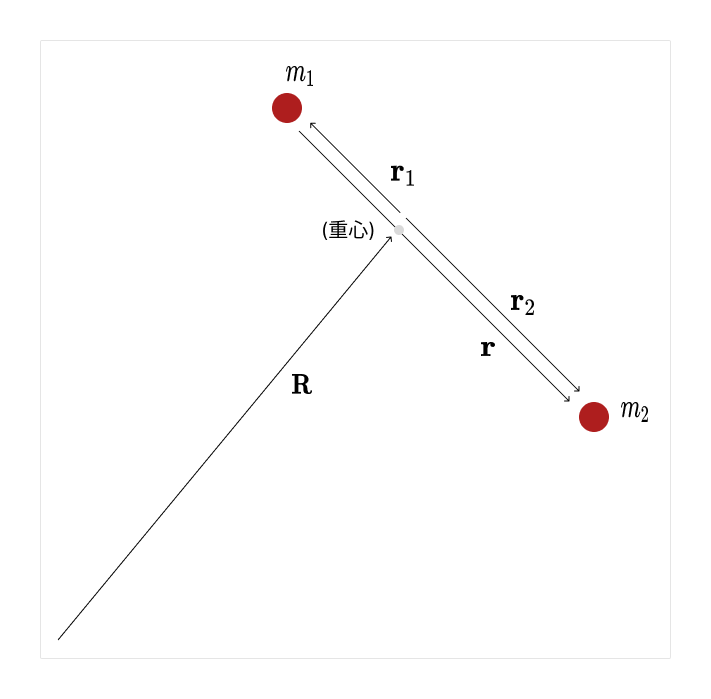
\includegraphics[width=.60\columnwidth]{./images/two_body_initial.png}\\
\noindent
質量$m_1$、質量$m_2$の2つの物質が相互作用しながらどのように運動するかを考える。\\
図のような状態を想定すると、
\begin{eqnarray*}
	\bm{r_1} &=& - \frac{m_2}{m_1+m_2} \bm{r}\\
	\bm{r_2} &=& \frac{m_1}{m_1+m_2} \bm{r}
\end{eqnarray*}
系自体の運動エネルギーが
$$ \frac{1}{2} (m_1+m_2) \dot{ \bm{R} }^2 $$
$m_1$、$m_2$それぞれの運動エネルギーが
\begin{eqnarray*}
	\frac{1}{2} m_1 \biggl{(} - \frac{m_2}{m_1+m_2} \biggr{)}^2  \dot{ \bm{r} }\\
	\frac{1}{2} m_2 \biggl{(} \frac{m_1}{m_1+m_2} \biggr{)}^2  \dot{ \bm{r} }
\end{eqnarray*}
よって、全体の運動エネルギーは
$$
T = \frac{1}{2} (m_1+m_2) \dot{ \bm{R} }^2 + \frac{1}{2} \biggl{(} \frac{m_1m_2}{m_1+m_2} \biggr{)}^2 \dot{ \bm{r} }^2
$$
ここで、系と同じ速度で動く座標系で考えると$\dot{ \bm{R} }= 0$で\\
$$m = \frac{m_1m_2}{m_1+m_2}$$
を導入すると
$$T = \frac{1}{2} m \dot{ \bm{r} }^2$$
これを極座標に変換し、さらにこの運動のラグラジアンを考える。\\
2物質の相互作用によるエネルギー$V(r)$とおくと\\
\begin{eqnarray*}
	L = \frac{1}{2} m ( \dot{r}^2 + r^2 \dot{ \theta }^2 ) - V(r)
\end{eqnarray*}
\begin{tcolorbox}
$r$についてオイラーラグランジュ方程式を考えて\\
\begin{eqnarray}
	\frac{ \partial L }{ \partial r } - \frac{d}{dt} \biggl{(} \frac{\partial L}{\partial \dot{r}}  \biggr{)} &=& 0 \nonumber \\
	mr \dot{\theta}^2 - \frac{ \partial V }{ \partial r } - m \ddot{r} &=& 0
\end{eqnarray}
\end{tcolorbox}
\begin{tcolorbox}
$\theta$についてもオイラーラグランジュ方程式を考えて\\
$$
\frac{ \partial L }{ \partial \theta } - \frac{d}{dt} \biggl{(} \frac{\partial L}{\partial \dot{\theta}}  \biggr{)} = 0
$$
ここで、$\frac{ \partial L }{ \partial \theta } = 0$より、
\begin{eqnarray}
	mr^2\dot{ \theta } = l = const.
\end{eqnarray}
\end{tcolorbox}
\begin{tcolorbox}
エネルギー保存則より、即座に
\begin{eqnarray}
	\frac{1}{2} m \dot{r}^2 + \biggl{(} \frac{1}{2} \frac{l^2}{mr^2} + V(r) \biggr{)} = E = const.
\end{eqnarray}
\end{tcolorbox}

\subsection{
ケプラー問題の解
}
$(2.5)$、$(2.6)$式を用いて、実際にケプラー問題を解いてみる。\\
$$ \frac{1}{2} \frac{l^2}{mr^2} + V(x) = V' $$
とおくと、$(2.5)$より
$$ \frac{dr}{dt} = \sqrt{ \frac{2(E-V')}{m} } $$
(2.6)より
$$ \frac{d\theta}{dt} = \frac{l}{mr^2}$$
よって
$$
\frac{dr}{d\theta} = \frac{ r^2 \sqrt{2m(E-V')} }{l}
$$
以上より、ケプラー問題は以下の積分を解くことに帰着された。
\begin{tcolorbox}
\begin{eqnarray*}
	\theta = \int_{r_0}^{r} \frac{l}{r^2 \sqrt{2m(E-V')} } dr + \theta'
\end{eqnarray*}
\end{tcolorbox}
\noindent
この問題は$V(x) = - \frac{k}{r}$のとき、解くことができるので、実際にやってみる。\\
$V'$を展開し、$\mu = \frac{1}{r}$とおくと
$$ \theta = \int_{\mu_0}^{\mu} \frac{1}{ \sqrt{ -\biggl{(} \mu - \frac{mk}{l} \biggr{)}^2 + \biggl{(} \frac{mk}{l} \biggr{)}^2 \biggl{(} 1 + \frac{2E}{mk^2} \biggr{)} } } d\mu + \theta'$$
$\alpha = \frac{l}{mk}$、$\beta = \sqrt{ 1 + \frac{2E}{mk^2} }$とおくと
\begin{eqnarray*}
    \theta &=& \int_{\mu_0}^{\mu}
    \frac{1}{ \sqrt{ -\left( \mu - \frac{1}{\alpha} \right)^2 + \left( \frac{\beta}{\alpha} \right)^2 } }
    d\mu + \theta' \\
    &=& \int_{\mu_0}^{\mu}
    \frac{1}{ \frac{\beta}{\alpha} \sqrt{ 1 - \left( \frac{ \mu - \frac{1}{\alpha} }{ \frac{\beta}{\alpha} } \right)^2 } }
    d\mu + \theta'
\end{eqnarray*}
$\cos{\gamma} = \left( \frac{ \mu - \frac{1}{\alpha} }{ \frac{\beta}{\alpha} } \right) $とおくと
\begin{eqnarray*}
    \theta -  \theta' &=& \int_{\gamma_0}^{\gamma} - d\gamma + \theta' \\
    &=& \gamma - \gamma '
\end{eqnarray*}
$\gamma_0 = 0$になるような$r_0$を基準に考えれば
\begin{eqnarray*}
    \theta - \theta' &=& - \gamma \\
    &=& - \cos^{-1} \left( \frac{ \mu - \frac{1}{\alpha} }{ \frac{\beta}{\alpha} } \right) \\
    \frac{\beta}{\alpha} \cos{(\theta - \theta')} &=& \mu - \frac{1}{\alpha} \\
    \frac{mk}{l} \sqrt{ 1 + \frac{2E}{mk^2} } \cos{(\theta - \theta')} &=& \frac{1}{r} - \frac{mk}{l}
\end{eqnarray*}
したがって、最終的には
\begin{tcolorbox}
\begin{eqnarray*}
	\frac{1}{r} = \frac{mk}{l} \left( 1 + \sqrt{ 1 + \frac{2E}{mk^2} } \cos{( \theta - \theta' )} \right)
\end{eqnarray*}
\end{tcolorbox}
\noindent
と求めることができた。


\chapter{2024 05/29}
% =================================
% chapter 3
% =================================

\section{
    測地線方程式の導出
}
一般の空間上での任意の2点$ P_1$と$P_2$を結ぶ最短経路を考える。\\
これは、あらゆる可能な経路の中からその長さが最小となるものを取り出せば良い。\\
まずは一般の経路$S$を考える。
$$
S = \int_{P_1}^{P_2} {ds}
$$
パラメータ$\lambda$を用いて
\begin{eqnarray*}
S &=& \int_{\lambda_1}^{\lambda_2} \frac{ ds }{ d\lambda } d\lambda \\
&=& \int_{\lambda_1}^{\lambda_2} d\lambda \sqrt{ g_{\mu \upsilon}(x) \frac{ dx^{\mu} }{ d\lambda }\frac{ dx^{\upsilon} }{ d\lambda } }
\end{eqnarray*}
作用が最小になる点でオイラーラグランジュ方程式を得るので、
$$
L\left( x^\mu, \frac{ dx^\mu }{ d\lambda } \right) = \sqrt{ g_{\mu \upsilon}(x) \frac{ dx^{\mu} }{ d\lambda }\frac{ dx^{\upsilon} }{ d\lambda } }
$$
とおけば、任意の$\alpha$に対して
$$
\frac{ \partial L }{ \partial x^\alpha } - \frac{ d }{ d \lambda } \frac{ \partial L }{ \partial \dot{x}^\alpha } = 0
$$
が成り立つ。
$$f = g_{\mu \upsilon}(x) d \dot{x}^{\mu} d \dot{x}^{\upsilon} $$
とおくと
\begin{eqnarray}
\frac{ \partial L }{ \partial x^\alpha } &=& \frac{ \partial L }{ \partial f } \frac{ \partial f }{ \partial x^\alpha } \nonumber \\
&=& \frac{ g_{\mu \upsilon , \alpha} \dot{x^\mu} \dot{x^\upsilon} }{ 2\sqrt{ g_{\mu \upsilon} \dot{x^\mu} \dot{x^\upsilon} } }
\end{eqnarray}
\begin{eqnarray}
\frac{ d }{ d\lambda } \frac{ \partial L }{ \partial \dot{x}^\alpha } &=& \frac{d}{d \lambda} \left( \frac{1}{2} f^{ - \frac{1}{2} } \right) \left( \frac{ g_{\mu \upsilon} \dot{x^\mu} \dot{x^\upsilon} }{ \partial \dot{x}^\alpha } \right) \nonumber \\ 
&=& \frac{d}{d \lambda} \left( \frac{1}{2} f^{ - \frac{1}{2} } \right) \left( g_{\mu \upsilon} \tensor{\delta}{^\mu_\alpha} \dot{x}^\upsilon + g_{\mu \upsilon} \tensor{\delta}{^\upsilon_\alpha} \dot{x}^\mu \right)\nonumber \\
&=& \frac{d}{d\lambda} \left( \frac{ g_{\alpha \upsilon}\dot{x}^{\upsilon} }{ \sqrt{g_{\mu \upsilon}\dot{x}^{\upsilon}  \dot{x}^{\upsilon} } } \right)
\end{eqnarray}
$(3,1)$$(3,2)$より、オイラーラグランジュ方程式は
$$
 \frac{ g_{\mu \upsilon , \alpha} \dot{x^\mu} \dot{x^\upsilon} }{ 2\sqrt{ g_{\mu \upsilon} \dot{x^\mu} \dot{x^\upsilon} } } - \frac{d}{d\lambda} \left( \frac{ g_{\alpha \upsilon}\dot{x}^{\upsilon} }{ \sqrt{g_{\mu \upsilon}\dot{x}^{\upsilon}  \dot{x}^{\upsilon} } } \right) = 0
$$
と書き換えられる。\\
$h = g_{\mu \upsilon}\dot{x}^{\mu}  \dot{x}^{\upsilon}$とおくと
\begin{eqnarray*}
 \frac{ g_{\mu \upsilon , \alpha} \dot{x^\mu} \dot{x^\upsilon} }{ 2\sqrt{ g_{\mu \upsilon} \dot{x^\mu} \dot{x^\upsilon} } } - \left( \frac{1}{2} h^{- \frac{3}{2}} \right) \dot{h} g_{\alpha \upsilon} \dot{x}^{\upsilon} - h^{- \frac{1}{2}} g_{\alpha \upsilon} \ddot{x}^{\upsilon} - h^{- \frac{1}{2}} g_{\alpha \upsilon, l} \dot{x}^l \dot{x}^{\upsilon} &=& 0 \nonumber \\
\end{eqnarray*}
$h^{\frac{1}{2}}g^{\epsilon \alpha}$をかけると
\begin{eqnarray*}
 \frac{1}{2} g^{\epsilon \alpha} g_{\mu \upsilon , \alpha} \dot{x^\mu} \dot{x^\upsilon} - 
\left( \frac{1}{2} h^{-1} \right) \dot{h} g^{\epsilon \alpha} g_{\alpha \upsilon} \dot{x}^{\upsilon} - g^{\epsilon \alpha} g_{\alpha \upsilon} \ddot{x}^{\upsilon} - g^{\epsilon \alpha} g_{\alpha \upsilon, l} \dot{x}^l \dot{x}^{\upsilon} &=& 0 \nonumber \\
\ddot{x}^{\epsilon} + \frac{1}{2} \dot{x^\mu} \dot{x^\upsilon} g^{\epsilon \alpha} \left( g_{\alpha \upsilon, l} + g_{\alpha l, \upsilon} - g_{\mu \upsilon , \alpha} \right) &=&
- \left( \frac{1}{2} h^{-1} \right) \dot{h} g^{\epsilon \alpha} g_{\alpha \upsilon} \dot{x}^{\upsilon}
\end{eqnarray*}
ここで、適切な間隔$\lambda$を用いると、$\dot{h} = 0$となるので
\begin{eqnarray*}
\ddot{x}^{\epsilon} + \frac{1}{2} \dot{x^\mu} \dot{x^\upsilon} g^{\epsilon \alpha} \left( g_{\alpha \upsilon, l} + g_{\alpha l, \upsilon} - g_{\mu \upsilon , \alpha} \right) &=& 0
\end{eqnarray*}
クリストッフェル記号を導入すると
\begin{eqnarray*}
\ddot{x}^{\epsilon} + \Gamma^{\alpha}_{\; l \upsilon} \dot{x}^l \dot{x}^{\upsilon} = 0
\end{eqnarray*}
\begin{tcolorbox}[title=測地線方程式]
\begin{eqnarray*}
\frac{ \partial ^2 {x}^{\epsilon} }{ \partial \lambda^2 } + \tensor{\Gamma}{^{\alpha}_{l \upsilon}} \frac{ \partial x^l }{ \partial \lambda } \frac{ \partial x^{\upsilon} }{ \partial \lambda } &=& 0
\end{eqnarray*}
\end{tcolorbox}

\section{
    クリストッフェル記号
}
あるベクトル場において、位置$x^i$でのベクトル$A^{i}(x)$と、そこから$\delta x^i$だけズレた位置でのベクトル$A^{i}(x+\delta x)$を比較することを考える。\\
しかし、無限小といえども異なる2点でのベクトルの値をそのまま比較することには幾何学的な意味がないため、この比較には座標普遍な方法が必要である。\\
その方法が並行移動である。\\
ベクトル$A^{i}(x)$を$\delta x^i$だけズレた位置に並行移して得られるベクトルを以下のように定義する。
$$
\tilde{A}^{i} (x+\delta x) := A^{i}(x) - \tensor{\Gamma}{^i_{jk}}(x) A^{j}(x) \delta x^{k}
$$
ここで、現れる係数$\tensor{\Gamma}{^i_{jk}}$を接続と呼ぶ。
\subsection{
	座標変換に対応した接続の変換
}
まずは座標が$x$から$\bar x$に変換した際の接続の変換を考える。\\
すると、並行移動は以下のように定義される。
$$
\tilde{ \bar{A} }^{l} (\bar{x}+\delta \bar{x}) := \bar{A}^{l}(\bar{x}) - \tensor{ \bar{\Gamma} }{^l_{mn}}(\bar{x}) \bar{A}^{m}(\bar{x}) \delta \bar{x}^{n}
$$
$\bar{A}^l$と$\tilde{ \bar{A} }^l$がそれぞれ反変ベクトルとして変換することを考慮すると
\begin{tcolorbox}
\begin{eqnarray}
\tilde{ \bar{A} }^{l} (\bar{x}+\delta \bar{x}) = \left. \frac{\partial \bar{x}^l }{ \partial x^i } \right|_{x+\delta x} \tilde{A}^i(x+\delta x)
\end{eqnarray}
ここで
\begin{eqnarray*}
\left. \frac{\partial \bar{x}^l }{ \partial x^i } \right|_{x+\delta x} = \frac{ \partial \bar{x}^l }{ \partial x^i } + \frac{ \partial \left( \frac{ \partial \bar{x}^l }{ \partial x^i } \right)  }{ \partial x^k }\delta x^k + ...
\end{eqnarray*}
\end{tcolorbox}
\begin{tcolorbox}
\begin{eqnarray}
\bar{A}^{l} (\bar{x}) = \frac{\partial \bar{x}^l }{ \partial x^i } A^i(x)
\end{eqnarray}
\end{tcolorbox}
$\delta \bar{x}^n = \frac{d\bar{x}^n}{dt}$とおけば、$\delta \bar{x}^n$反変ベクトルと考えることができるので
\begin{tcolorbox}
\begin{eqnarray}
\delta \bar{x}^n = \frac{\partial \bar{x}^n}{\partial x^k} \delta x^k(x)
\end{eqnarray}
\end{tcolorbox}
$(3.3),(3.4),(3.5)$と並行移動の定義より\\
\begin{eqnarray*}
\left( \frac{ \partial \bar{x}^l }{ \partial x^j } + \frac{ \partial^2 \bar{x}^l }{ \partial x^k \partial x^j }\delta x^k + ... \right) \left( A^j - \tensor{\Gamma}{^i_{jk}} A^j(x) \delta x^k \right) = \\
\frac{ \partial \bar{x}^l }{ \partial x^i }A^i(x) - \tensor{\bar{ \Gamma }}{^l_{mn}} \left( \frac{\partial \bar{x}^m}{\partial x^i} A^i(x) \right) \left( \frac{\partial \bar{x}^n}{\partial x^k} \delta x^k \right)
\end{eqnarray*}
$\delta x^k$がある項に注目すると、
\begin{eqnarray*}
\frac{\partial^2 \bar{x}^l}{\partial x^k \partial x^j} \delta x^k A^j(x) - \tensor{\Gamma}{^i_{jk}} \frac{\partial \bar{x}^l}{\partial x^i}A^j(x) \delta x^k = \\
- \tensor{\bar{\Gamma}}{^l_{mn}} \frac{\partial \bar{x}^m}{\partial x^j} \frac{\partial \bar{x}^n}{\partial x^k}\delta x^k A^j(x)
\end{eqnarray*}
両辺に$\frac{\partial x^i}{\partial \bar{x}^l}$をかけると
\begin{tcolorbox}
\begin{eqnarray*}
\frac{\partial^2 \bar{x}^l}{\partial x^k \partial x^j} \frac{\partial x^i}{\partial \bar{x}^l} - \tensor{\Gamma}{^i_{jk}} = - \tensor{\bar{\Gamma}}{^l_{mn}} \frac{\partial \bar{x}^m}{\partial x^j} \frac{\partial \bar{x}^n}{\partial x^k} \frac{\partial x^i}{\partial \bar{x}^l}
\end{eqnarray*}
\end{tcolorbox}

\subsection{
	対称な接続
}
接続の条件として、並行移動によってベクトルの大きさと任意の2つのベクトルのなす角が普遍に保たれることを要求する。\\
これは任意の2つのベクトルの内積が普遍であることを意味する。\\
\begin{eqnarray*}
g_{ij} A^i(x)B^j(x) &=& g_{ij}(x + \delta x) \tilde{A}^i(x+\delta x) \tilde{B}^j(x+\delta x)\\
&=& (g_{ij} + g_{ij,k}\delta x^k)(A^i(x) - \tensor{\Gamma}{^i_{lk}}A^l(x) \delta x^k) (B^j(x) - \tensor{\Gamma}{^j_{lk}}B^l(x) \delta x^k)\\
&=& g_{ij} A^i(x)B^j(x) + (g_{ij,k} - g_{lj}\tensor{\Gamma}{^l_{ik}} - g_{il}\tensor{\Gamma}{^l_{jk}} )A^i B^j \delta x^k + O((\delta x)^2)
\end{eqnarray*}
これが任意の$A^i, B^j, \delta x^k$に対して成り立つためには
\begin{eqnarray*}
 g_{ij,k} - g_{lj}\tensor{\Gamma}{^l_{ik}} - g_{il}\tensor{\Gamma}{^l_{jk}} = 0
 \end{eqnarray*}
 ここで、対称な接続
\begin{eqnarray}
\tensor{\Gamma}{^l_{jk}} = \tensor{\Gamma}{^l_{kj}}
\end{eqnarray}
 を満たす接続のみを考えると
\begin{eqnarray}
 g_{ij,k} - g_{jl}\tensor{\Gamma}{^l_{ik}} - g_{il}\tensor{\Gamma}{^l_{jk}} &=& 0\\
 g_{ik,j} - g_{kl}\tensor{\Gamma}{^l_{ij}} - g_{il}\tensor{\Gamma}{^l_{kj}} &=& 0\\
 - g_{kj,i} + g_{jl}\tensor{\Gamma}{^l_{ki}} + g_{kl}\tensor{\Gamma}{^l_{ji}} &=& 0
\end{eqnarray}
$(3.6), (3.7), (3.8), (3.9)$より
\begin{tcolorbox}[title=クリストッフェル記号]
\begin{eqnarray*}
	\tensor{\Gamma}{^i_{jk}} = \frac{1}{2} g^{il} (g_{lj,k} + g_{lk,j} - g_{jk,l})
\end{eqnarray*}
\end{tcolorbox}

\chapter{2024 06/05}
% =================================
% chapter 4
% =================================

\section{
	シュワルツシルト時空における軌道の予測
}
\subsection{
	具体的な測地線方程式の導出
}

\[
ds^2 = -A(r)dt^2 + B(r)dr^2 + r^2d \theta^2 + r^2 \sin^2 \theta d\phi^2
\]
線素が以上のように表される、曲がった時空を考える。\\
測地線方程式を思い出すと
\[
\ddot{x}^{\epsilon} + \tensor{\Gamma}{^{\alpha}_{l \upsilon}} \dot{x}^l \dot{x}^{\upsilon} = 0
\]
このようになっているので、クリストッフェル記号の具体的な値を求めたい。\\
クリストッフェル記号は計量の微分で表現できたので、まずは計量の値を求める。\\
\[
x^{\mu} = ( t, r, \theta, \phi )
\]
とおくと、計量のゼロでない値は
\begin{equation*}
\begin{split}
g_{00} &= -A(r)\\
g_{11} &= B(r)\\
g_{22} &= r^2\\
g_{33} &= r^2 \sin^2 \theta
\end{split}
\end{equation*}
となっている。\\
続いて、計量の微分でゼロにならないものを考えると
\begin{equation*}
\begin{split}
g_{00,1} &= -A'(r)\\
g_{11,1} &= B'(r)\\
g_{22,1} &= 2r\\
g_{33,1} &= 2r \sin^2 \theta\\
g_{33,2} &= 2 r^2 \sin \theta \cos \theta
\end{split}
\end{equation*}
最後に、クリストッフェル記号の値を具体的に求める。\\
クリストッフェル記号は以下のように与えられていたことを思い出すと
\[
\tensor{\Gamma}{^i_{jk}} = \frac{1}{2} g^{il} (g_{lj,k} + g_{lk,j} - g_{jk,l})
\]
ゼロでない値は以下のようになっている。
\begin{align*}
\tensor{\Gamma}{^0_{01}} &= \frac{1}{2} \frac{1}{A(r)} A'(r) &
\tensor{\Gamma}{^1_{00}} &= \frac{1}{2} \frac{1}{B(r)} A'(r)\\
\tensor{\Gamma}{^1_{11}} &= \frac{1}{2} \frac{1}{B(r)} B'(r) &
\tensor{\Gamma}{^1_{22}} &= - \frac{r}{B(r)}\\
\tensor{\Gamma}{^1_{33}} &= - \frac{r \sin^2 \theta}{B(r)} &
\tensor{\Gamma}{^2_{21}} &= \frac{1}{r}\\
\tensor{\Gamma}{^2_{33}} &= - \sin \theta \cos \theta &
\tensor{\Gamma}{^3_{31}} &= \frac{1}{r}\\
\tensor{\Gamma}{^3_{32}} &= \frac{ \cos \theta }{ \sin \theta }
\end{align*}
これを考慮して、測地線方程式
\[
\ddot{x}^i = \tensor{\Gamma}{^i_{jk}} \dot{x}^j \dot{x}^k
\]
を考えると\\
$i=0$では
\begin{equation}
\ddot{t} + \frac{A'(r)}{A(r)} \dot{t} \dot{r} = 0
\end{equation}
$i=1$では
\begin{equation}
\ddot{r} + \frac{A'(r)}{2B(r)} \dot{t}^2 + \frac{B'(r)}{2B(r)} \dot{r}^2 - \frac{r}{B(r)}\dot{\theta}^2 - \frac{r\sin^2 \theta}{B(r)} \dot{\phi}^2= 0
\end{equation}
$i=2$では
\begin{equation}
\ddot{\theta} + \frac{2}{r} \dot{r} \dot{\theta} - \sin \theta \cos \theta \dot{\phi}^2 = 0
\end{equation}
$i=3$では
\begin{equation}
\ddot{\phi} + \frac{2}{r} \dot{r} \dot{\phi} + 2 \frac{\cos \theta}{\sin \theta} \dot{\theta} \dot{\phi} = 0
\end{equation}

\subsection{
	軌道の予測
}
導出した測地線方程式から、この時空における物体の運動を予測したい。\\
ただ、簡単に解くことはできないので、まずは解析的に軌道を予測する。\\
この時空は球対称なので、まずは運動が$\theta = \frac{\pi}{2}$に収まっていると仮定してみる。\\
 すると\\
 $(4.1)$は
\begin{equation}
\begin{split}
\ddot{t} + \frac{A'(r)}{A(r)} \dot{t} \dot{r} &= 0\\
A(r) \ddot{t} + A'(r) \dot{t} \dot{r} &= 0\\
\frac{d}{d \lambda} \left( A(r) \dot{t} \right) &= 0\\
A(r) \dot{t} &= E = const.\\
\end{split}
\end{equation}
$(4.4)$は
\begin{equation}
\begin{split}
\ddot{\phi} + \frac{2}{r} \dot{r} \dot{\phi} &= 0\\
r^2 \ddot{\phi} + 2 r \dot{r} \dot{\phi} &= 0\\
\frac{d}{d \lambda} \left( r^2 \dot{\phi} \right) &= 0\\
r^2 \dot{\phi} &= l = const.
\end{split}
\end{equation}
ここで、測地線方程式を導出した際に仮定した拘束条件
\[
\frac{ d }{ d \lambda }\left( g_{\mu \upsilon}\dot{x}^{\mu}  \dot{x}^{\upsilon} \right) = 0
\]
を思い出して
\[
g_{\mu \upsilon}\dot{x}^{\mu}  \dot{x}^{\upsilon} = -1
\]
とおく。するとこれは
\begin{equation}
\begin{split}
-A(r) \dot{t}^2 + B(r) \dot{r}^2 + r^2 \dot{\theta}^2 + r^2 \sin^2 \theta \dot{\phi}^2 &= -1\\
- \frac{E^2}{A(r)} + B(r) \dot{r}^2 + \frac{l^2}{r^2} &= -1
\end{split}
\end{equation}
と変形できる。さらに
\[
A(r) = 1- \frac{2M}{r}
\]
\[
B(r) = \frac{1}{1- \frac{2M}{r}}
\]
の場合について考えると$(4.7)$は
\begin{tcolorbox}
\[
\dot{r}^2 = E^2 - \left( - \frac{2M}{r^3} l^2 + \frac{l^2}{r^2} - \frac{2M}{r} + 1 \right)
\]
\end{tcolorbox}
\noindent
この式から軌道を予測する。\\
\begin{equation*}
\begin{split}
E^2 - \left( - \frac{2M}{r^3} l^2 + \frac{l^2}{r^2} - \frac{2M}{r} + 1 \right) \geq 0
\end{split}
\end{equation*}
より
\[f(r) = - \frac{2M}{r^3} l^2 + \frac{l^2}{r^2} - \frac{2M}{r} + 1\]
を解析することで$E$における$r$の収まるべき範囲が推測できる。\\
\begin{equation*}
\begin{split}
f \left( \frac{1}{s} \right) = - 2M l^2 s^3 + l^2 s^2 - 2M s + 1\\
f' \left( \frac{1}{s} \right) = - 6M l^2 s^2 + 2 l^2 s - 2M
\end{split}
\end{equation*}
より、関数$f$は判別式
\[D= \left( l - \sqrt{12}M \right) \left( l + \sqrt{12}M \right) \]
によって分類できる。
\begin{figure}[H]
    \centering
    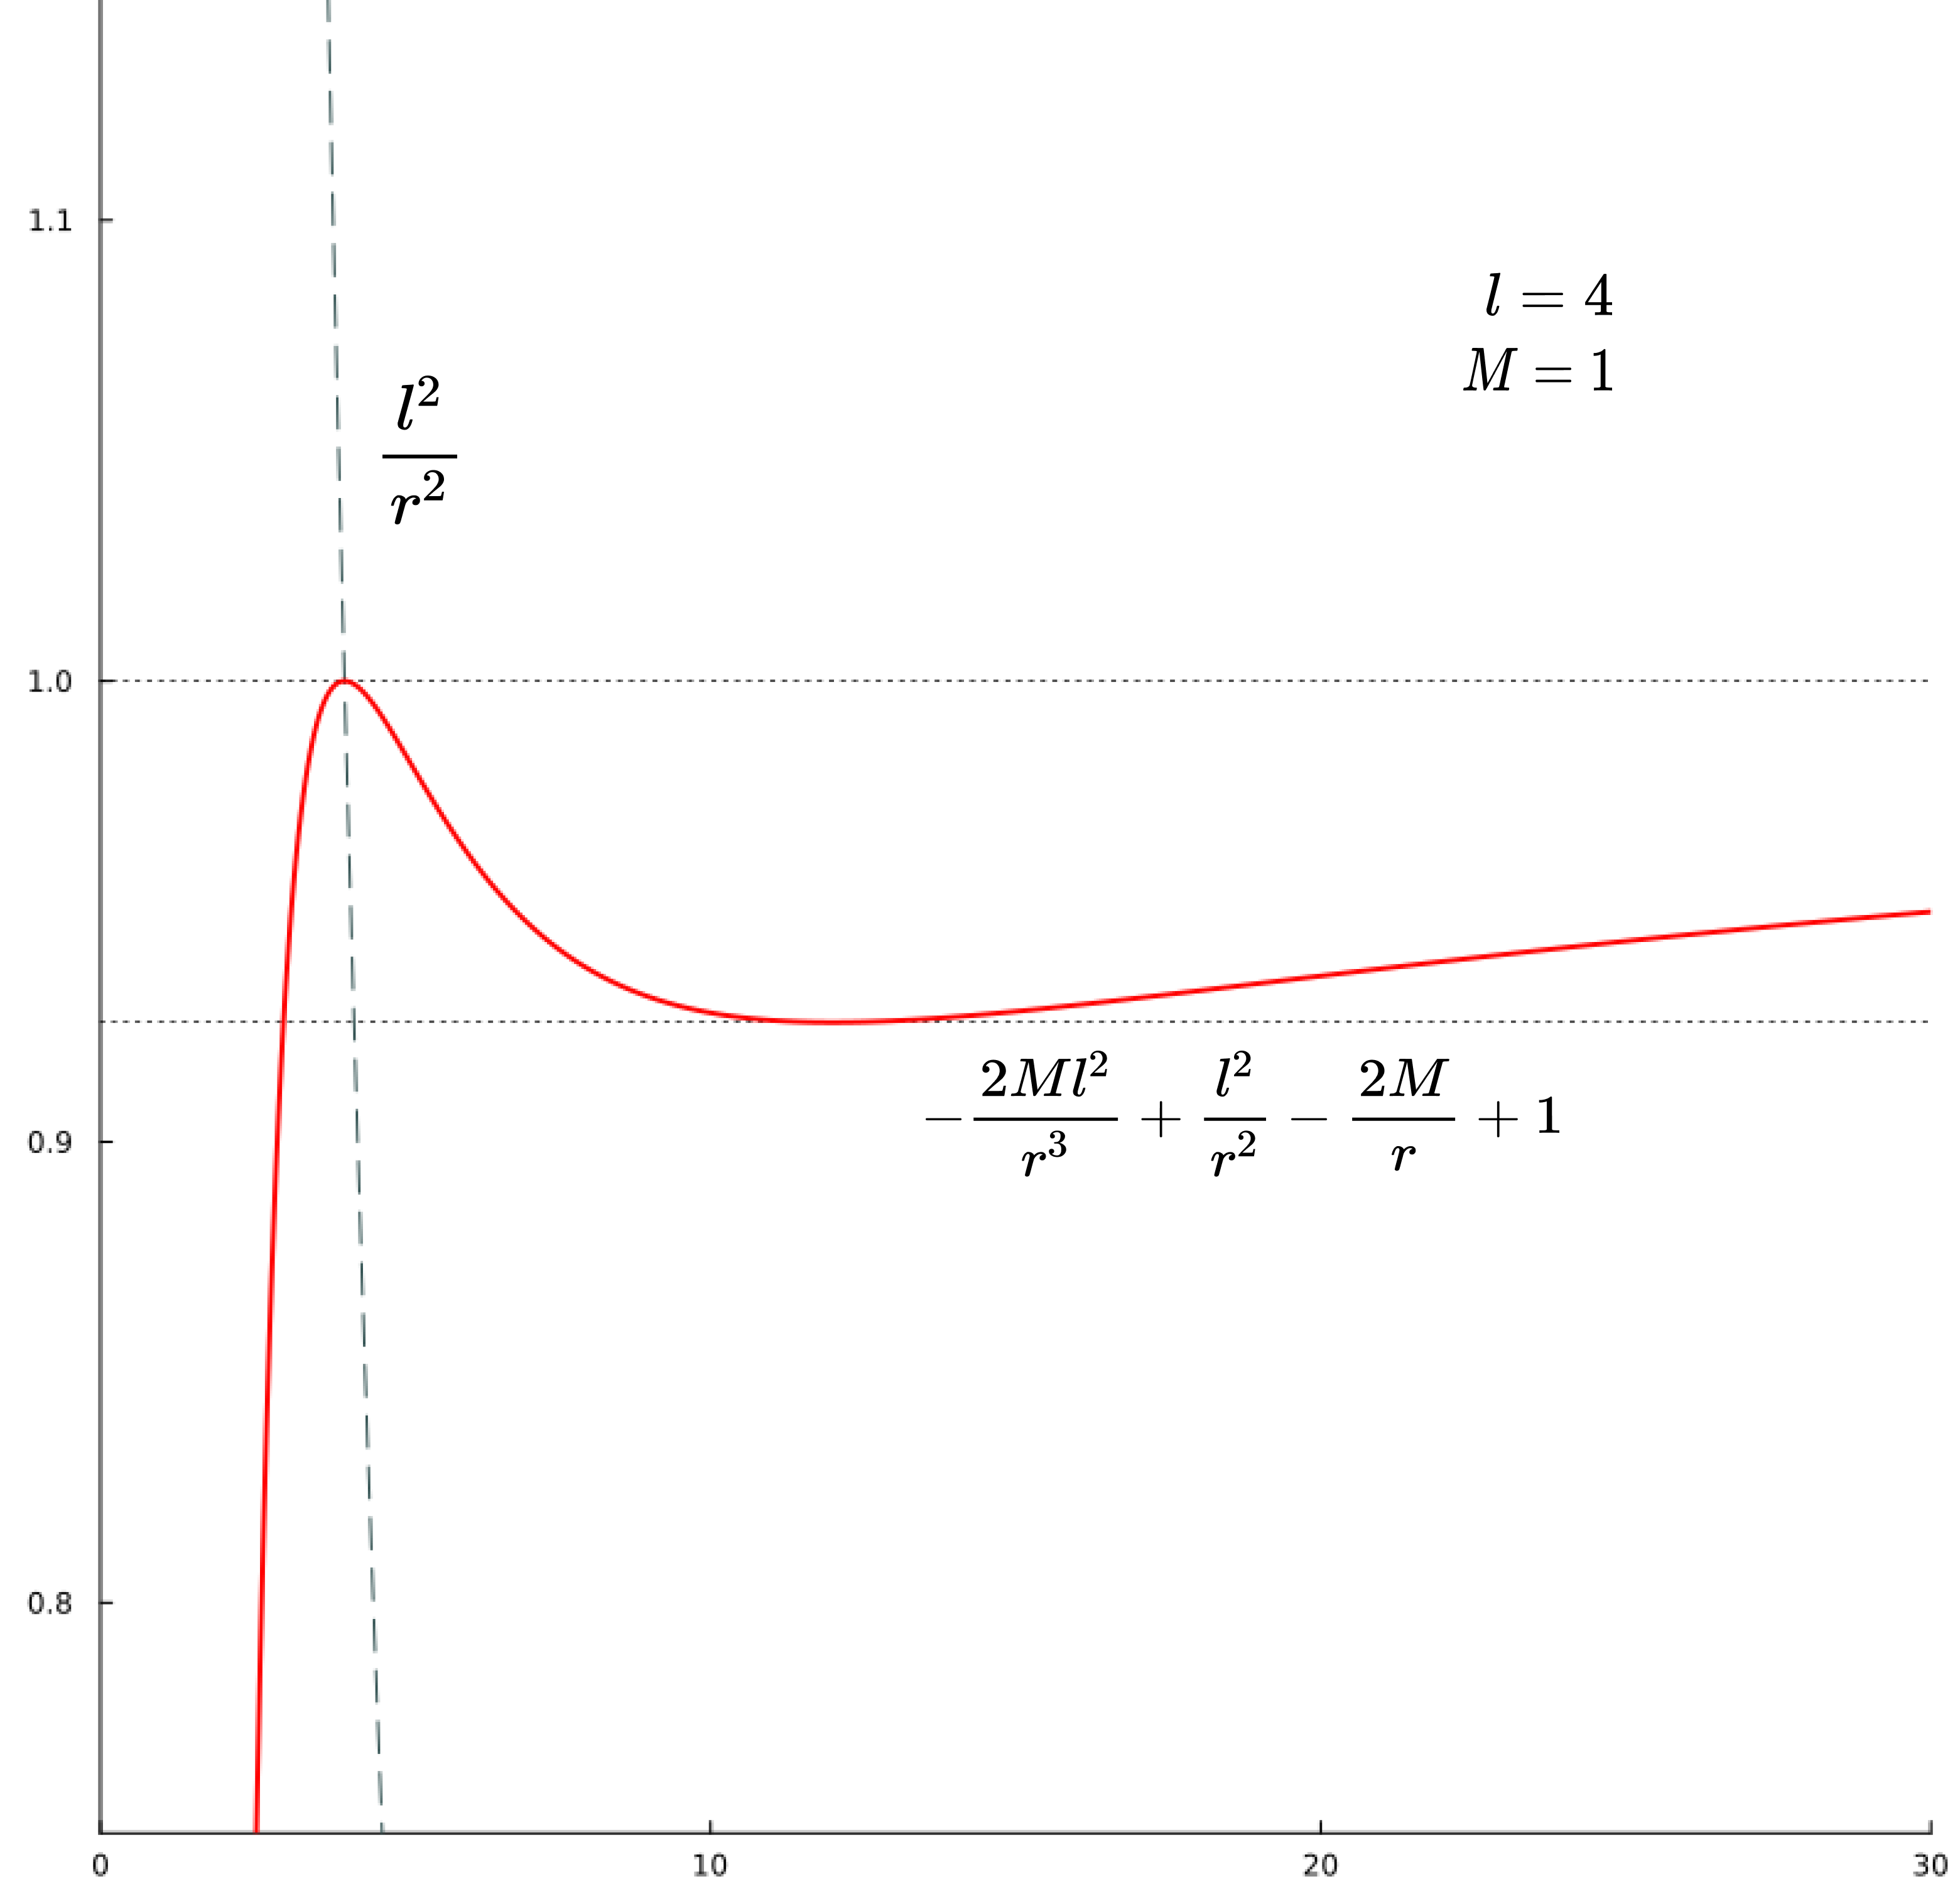
\includegraphics[width=0.5\columnwidth]{./images/schwarzschild/01.png}
    \caption{$D>0$}
    \label{01}
\end{figure}
\begin{figure}[H]
    \centering
    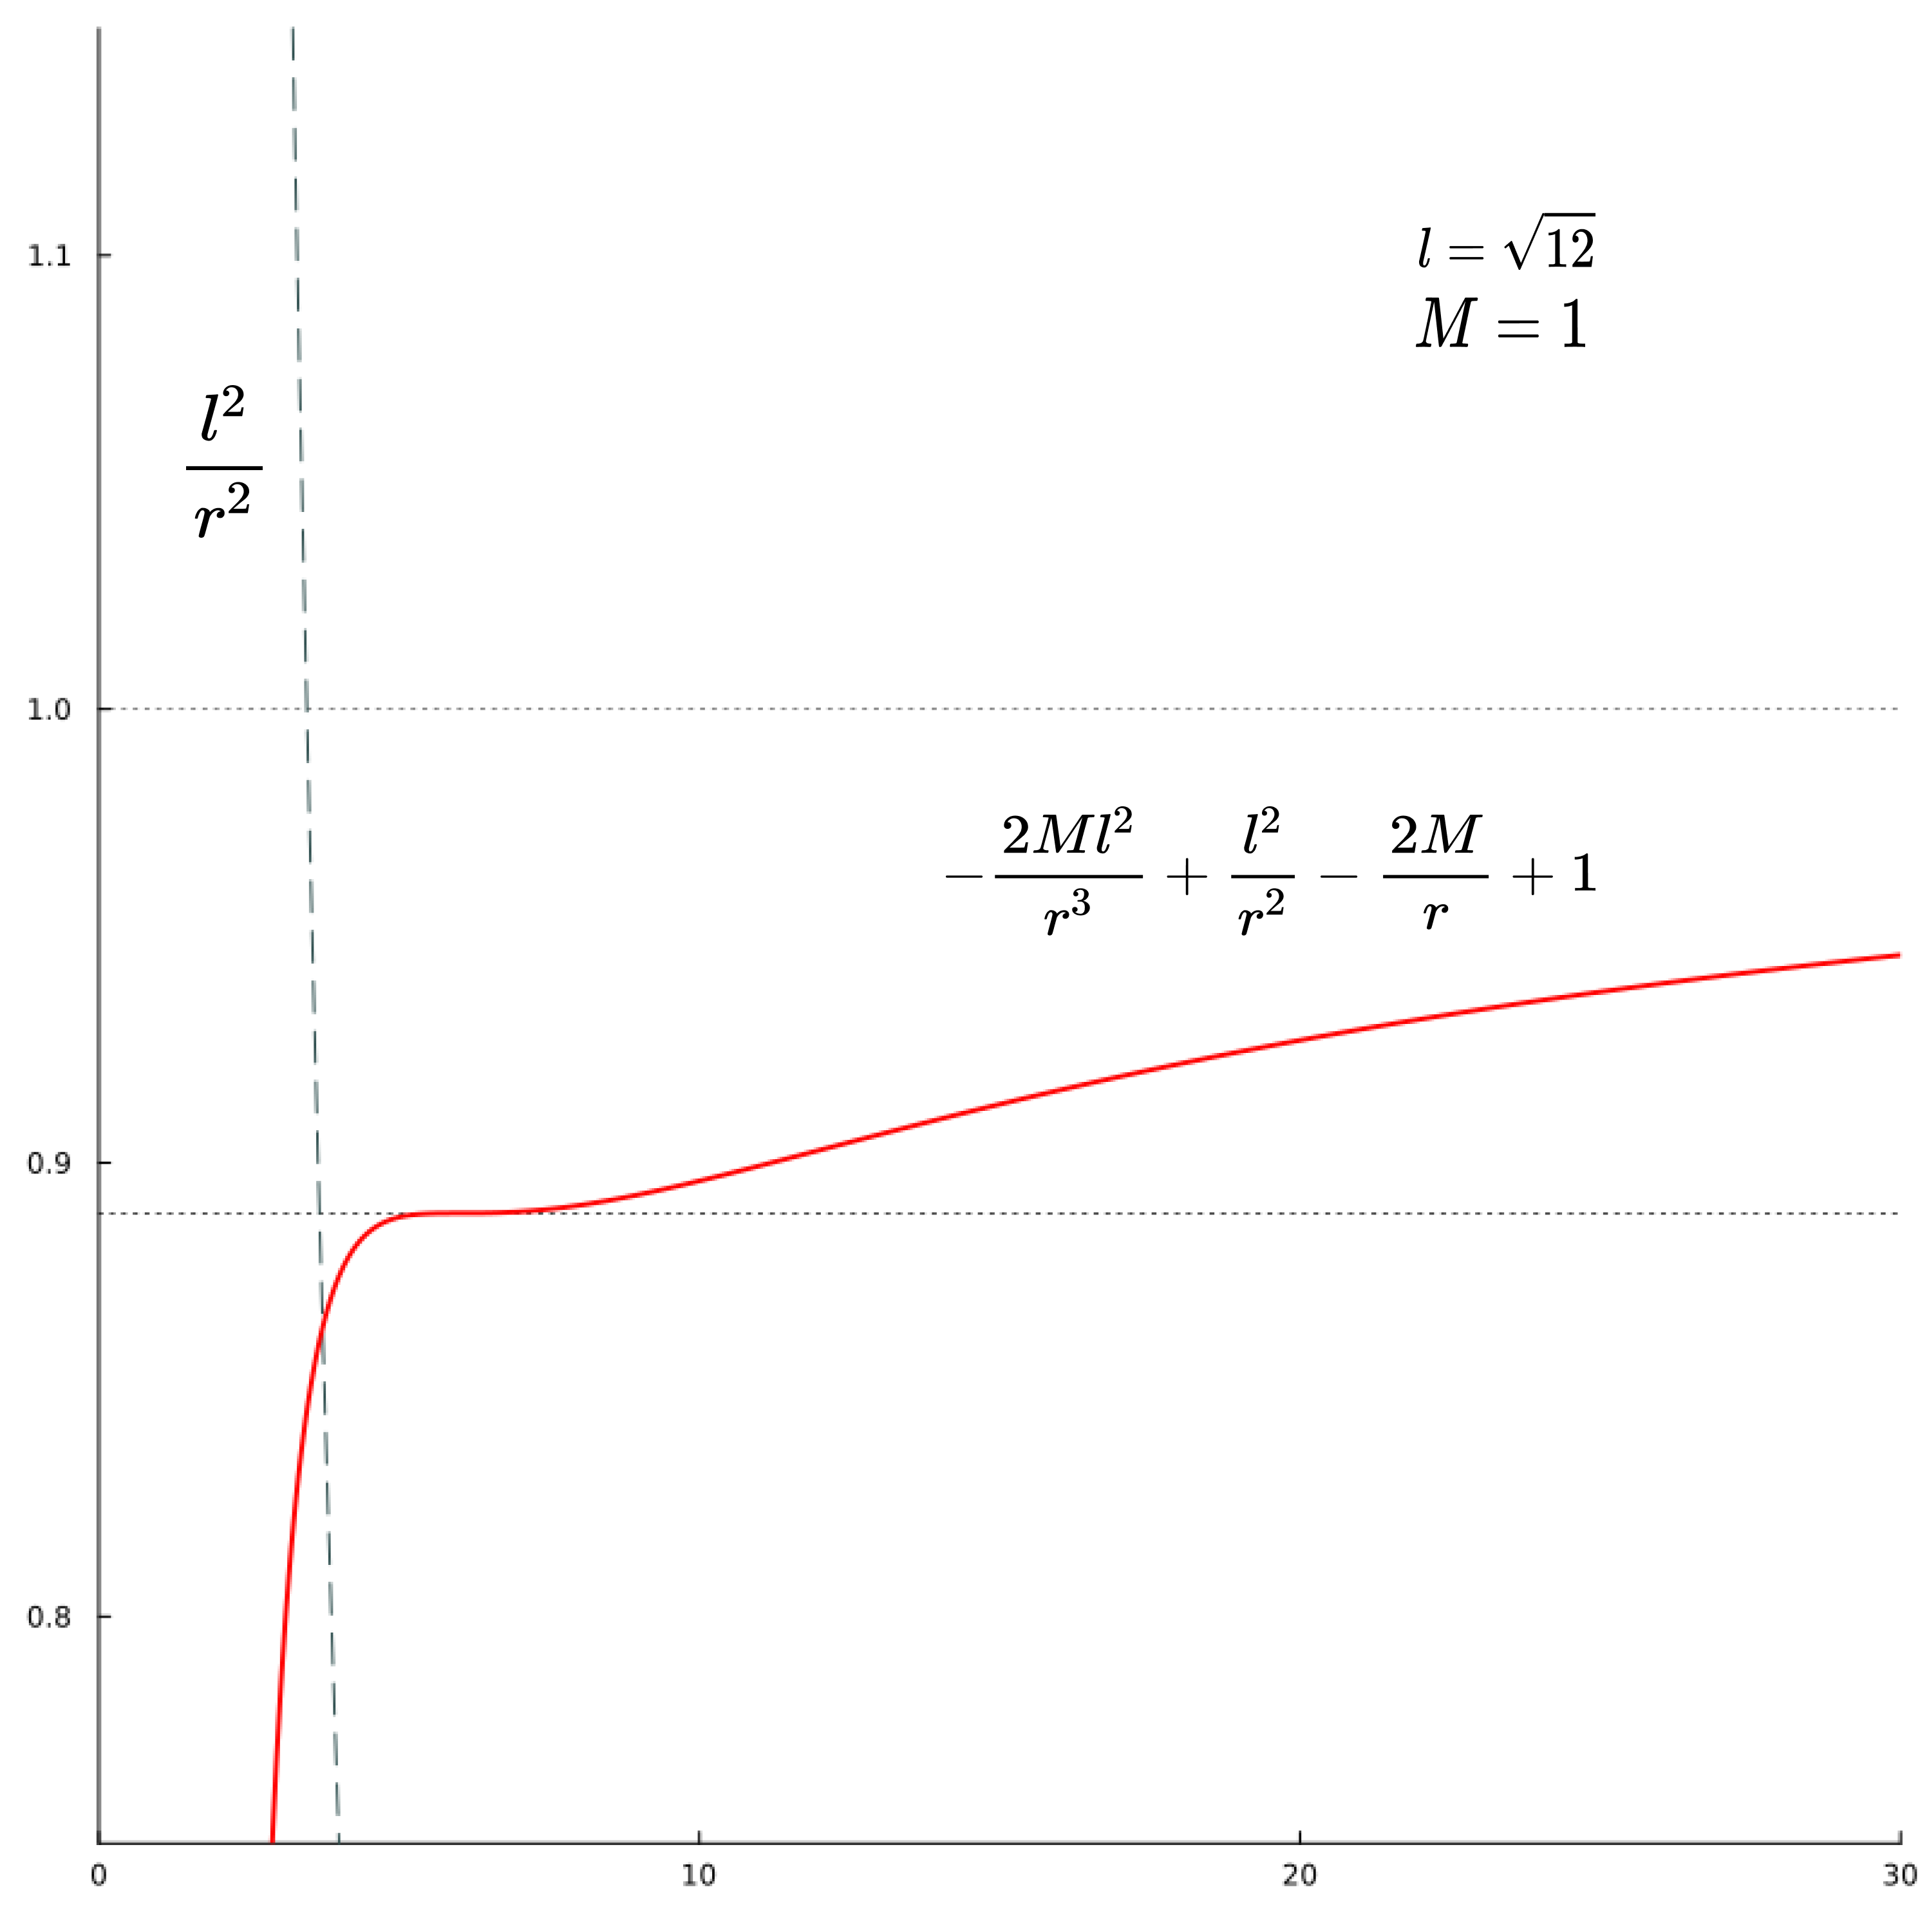
\includegraphics[width=0.5\columnwidth]{./images/schwarzschild/02.png}
    \caption{$D=0$}
    \label{02}
\end{figure}
\begin{figure}[H]
    \centering
    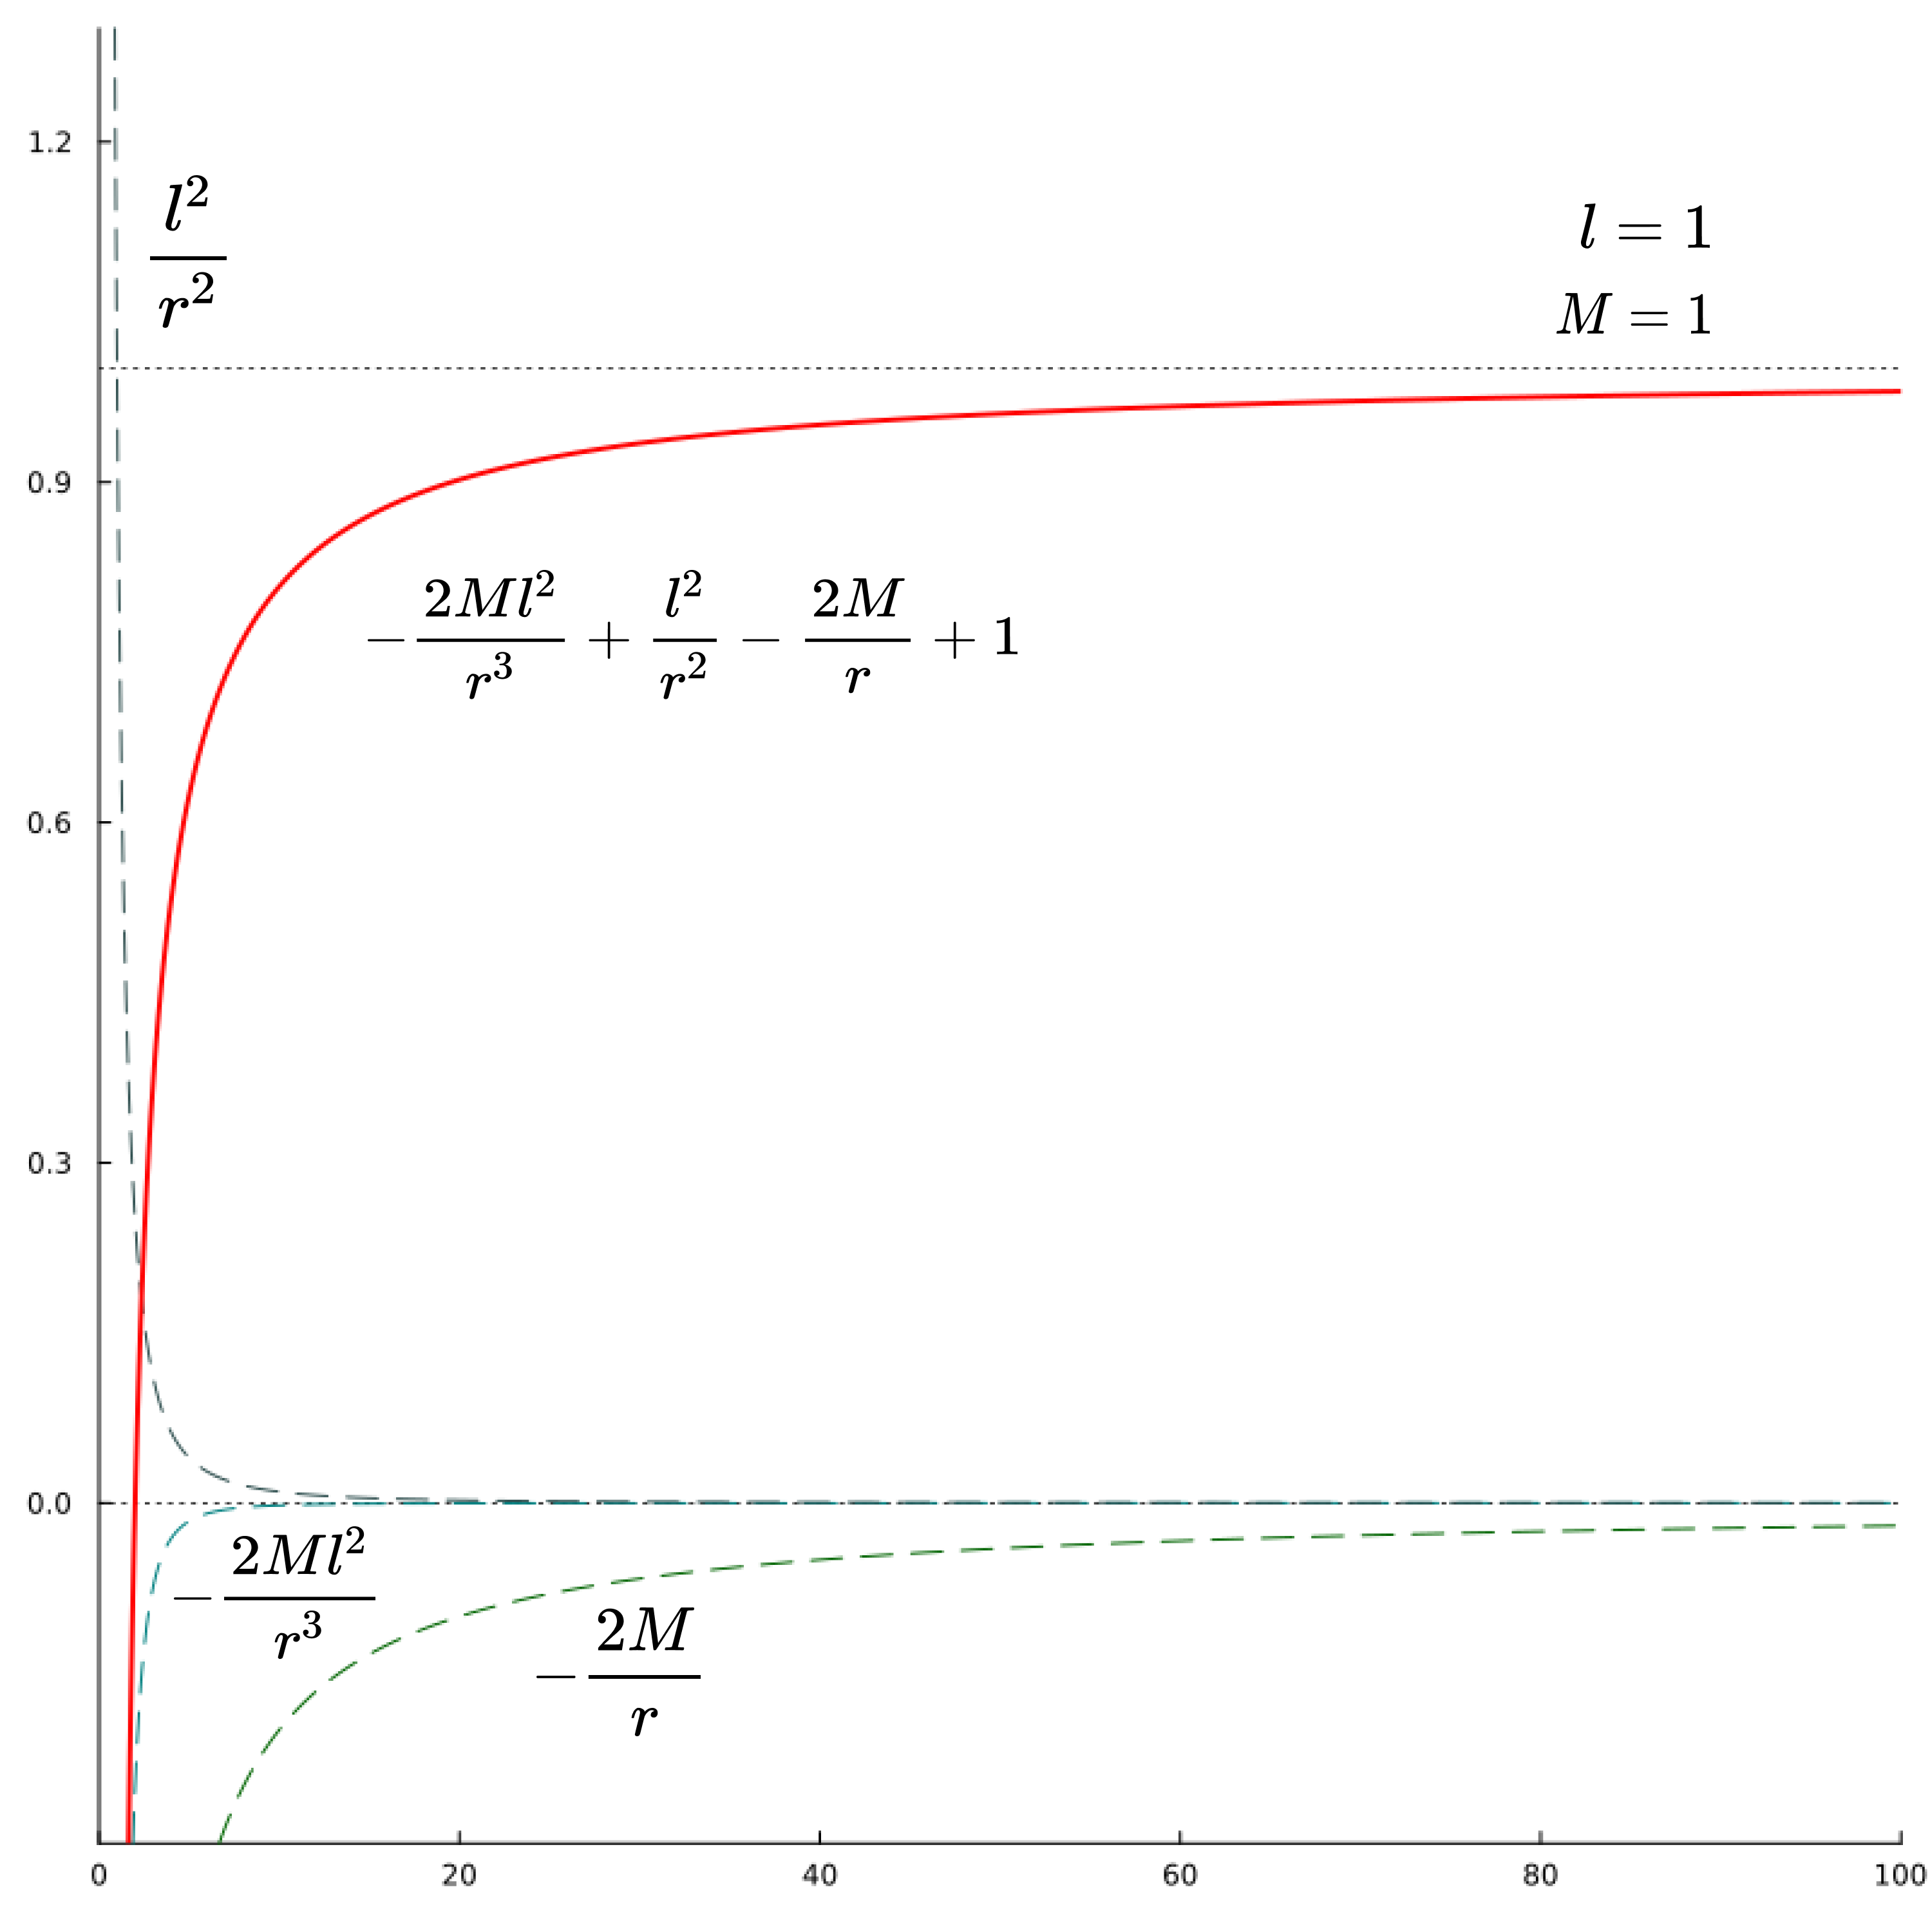
\includegraphics[width=0.5\columnwidth]{./images/schwarzschild/03.png}
    \caption{$D<0$}
    \label{03}
\end{figure}
\section{
    共変微分
}
反変ベクトルの偏微分に関しての座標変換を考えると
\begin{equation*}
\begin{split}
\frac{ \partial A^i(x) }{ \partial x^j } &= \frac{ \partial \bar{x}^l }{ \partial x^j } \frac{ \partial }{ \partial \bar{x}^l } \left( \frac{ \partial x^i }{ \partial \bar{x}^k } \bar{A}^k  \right)\\
&= \frac{\partial \bar{x}^l}{\partial{x}^j} \frac{\partial{x}^i}{\partial \bar{x}^k} \frac{\partial \bar{A}^k}{\partial \bar{x}^l} + \frac{\partial \bar{x}^l}{\partial x^j} \frac{\partial^2 x^i}{\partial \bar{x}^l \partial \bar{x}^k} \bar{A}^k
\end{split}
\end{equation*}
共変ベクトルの偏微分に関しての座標変換を考えると
\begin{equation*}
\begin{split}
\frac{ \partial A_i(x) }{ \partial x^j } &= \frac{ \partial \bar{x}^l }{ \partial x^j } \frac{ \partial }{ \partial \bar{x}^l } \left( \frac{ \partial \bar{x}^k }{ \partial x^i } \bar{A}_k  \right)\\
&= \frac{\partial \bar{x}^l}{\partial{x}^j} \frac{\partial \bar{x}^k}{\partial x^i} \frac{\partial \bar{A}^k}{\partial \bar{x}^l} + \frac{\partial \bar{x}^l}{\partial x^j} \frac{\partial^2 \bar{x}^k}{\partial \bar{x}^l \partial x^i} \bar{A}^k
\end{split}
\end{equation*}
以上より、これらはテンソルとしての変換性を持たない。\\
これは、無限小といえども異なる2点における座標は一般に異なっており、異なる2点でのベクトルを比較することは幾何学意味がないからである。\\
但し、並行移動を定義したことで、無現小異なる2点におけるベクトルを同一点に並行移動することによって、ベクトルの微分を同一点でのベクトルの差として表現することができる。\\
この無現小の差をとる演算子を$D$で表し、これがテンソルになるように、反変ベクトル、共変ベクトルそれぞれに対する共変微分を以下のように定義する。
\begin{tcolorbox}[title=反変ベクトルに対する共変微分]
\begin{equation*}
\begin{split}
\tensor{A}{^i_{;k}} \equiv \nabla_k A^i = \tensor{A}{^i_{,k}} + \Gamma^{i}_{jk}A^j
\end{split}
\end{equation*}
\end{tcolorbox}
\begin{tcolorbox}[title=共変ベクトルに対する共変微分]
\begin{equation*}
\begin{split}
\tensor{B}{_{i}_{;k}} \equiv \nabla_k B_i = \tensor{B}{_i_{,k}} + \Gamma^{i}_{jk}B_j
\end{split}
\end{equation*}
\end{tcolorbox}
最後に、一般のテンソルに対しての共変微分は、上のベクトルの場合を一般化して
\begin{tcolorbox}[title=一般のテンソルに対する共変微分]
\begin{equation*}
\begin{split}
\tensor{T}{^{i_1, i_2...i_k}_{j_1, j_2...j_l;q}} &= \tensor{T}{^{i_1, i_2...i_k}_{j_1, j_2...j_l,q}}\\
&+\sum^{k}_{m=1} \tensor{\Gamma}{^{i_m}_{pq}} \tensor{T}{^{i_1,i_2...i_{m-1},p,i_{m+1}...i_k}_{j_1, j_2...j_l}}\\
&+ \sum^{l}_{m=1} \tensor{\Gamma}{^{p}_{i_m q}} \tensor{T}{^{i_1,i_2...i_k}_{j_1, j_2...j_{m-1},p,j_{m+1}...j_l}}
\end{split}
\end{equation*}
\end{tcolorbox}
以上のように与えられる。

\section{
    リーマン曲率テンソル
}
等価原理により、どんな時空であれ局所的にはクリストッフェル記号がゼロになるような座標が存在する。\\
そこで、時空の曲がり具合を表現する共変的な量の導出が望ましい。\\
これがリーマンテンソルである。\\
曲がった時空上の4点$P, Q_1, Q_2, R$を考える。\\
点$P$から$\delta_1 x^i$だけズレた点を$Q_1$\\
点$P$から$\delta_2 x^i$だけズレた点を$Q_2$\\
点$Q_1$から$\delta_2 x^i$だけズレており、点$Q_2$から$\delta_1 x^i$だけズレてた点を$R$とする。\\
$P$で与えられたベクトル$A^i$を\\
$P \to Q_1 \to R$の順に並行移動したベクトルを
\[ \tilde{A}^i\left(R\right) \]
$P \to Q_2 \to R$の順に並行移動したベクトルを
\[ \tilde{A}'^i\left(R\right) \]
とおき、このベクトルのズレを空間の曲率と考えると、\\
これは$\delta_1 x^i, \delta_2 x^i$が無限小の場合、そのそれぞれ比例し、$A^i$にも比例していると考えられるので、\\
比例係数$\tensor{R}{^i_{jkl}}$を用いて
\begin{equation*}
\begin{split}
\delta A^i:=\tilde{A}^i\left(R\right)-\tilde{A}'^i\left(R\right)=R^i{}_{jkl} A^j \delta_1 x^k \delta_2 x^{l}
\end{split}
\end{equation*}
とかけるはずである。\\
この比例係数がリーマンテンソルである。\\
\begin{equation}
\begin{split}
\tilde{A}^i\left(R\right) =& \tilde{A}^i\left(Q_1\right)-\Gamma^i{}_{jk}\left(Q_1\right) \tilde{A}^j\left(Q_1\right) \delta_2 x^k \\
=& A^i-\Gamma^i{}_{jk} A^j\left(\delta_1 x^k+\delta_2 x^k\right) \\
& -\left(\Gamma^i{}_{j l, k}-\Gamma^i{}_{n l} \Gamma^n{}_{jk}\right) A^j \delta_1 x^k \delta_2 x^{l}
\end{split}
\end{equation}
\begin{equation}
\begin{split}
\tilde{A}'^i\left(R\right)= & \tilde{A}^i\left(Q_2\right)-\Gamma^i{}_{jk}\left(Q_2\right) \tilde{A}^j\left(Q_2\right) \delta_1 x^k \\
= & A^i-\Gamma^i{}_{jk} A^j\left(\delta_1 x^k+\delta_2 x^k\right) \\
& -\left(\Gamma^i{}_{jk, l}-\Gamma^i{}_{nk} \Gamma^n{}_{jl}\right) A^j \delta_1 x^k \delta_2 x^{l}
\end{split}
\end{equation}
$(4.8), (4.9)$より
\begin{tcolorbox}[title=リーマンテンソル]
\begin{equation*}
\begin{split}
\tensor{R}{^i_{jkl}} = \tensor{\Gamma}{^i_{jl,k}} - \tensor{\Gamma}{^i_{jk,l}} + \tensor{\Gamma}{^i_{nk}}\tensor{\Gamma}{^n_{jl}} - \tensor{\Gamma}{^i_{nl}}\tensor{\Gamma}{^n_{jk}}
\end{split}
\end{equation*}
\end{tcolorbox}\noindent
となっていることがわかる。

\chapter{2024 06/12}
% =================================
% chapter 5
% =================================
\section{
	共変微分とリーマンテンソル
}
共変微分とリーマンテンソルには以下のような関係性があるので、それを導出する。\\
\begin{equation*}
\begin{split}
	\nabla_a \nabla_b A_i &= \partial_a ( \nabla_b A_i ) - \Gamma^c_{ba}( \nabla_c A_i ) - \Gamma^c_{ia}( \nabla_b A_c ) \\
	&= \partial_a ( \partial_b A_i - \Gamma^c_{ib} A_c ) \\
	&\quad - \Gamma^c_{ba}( \partial_c A_i - \Gamma^d_{ic} A_d ) \\
	&\quad - \Gamma^c_{ia}( \partial_b A_c - \Gamma^d_{cb} A_d ) \\
	&= \partial_a \partial_b A_i - \partial_a \Gamma^c_{ib} A_c - \Gamma^c_{ib} \partial_a A_c \\
	&\quad - \Gamma^c_{ba} \partial_c A_i + \Gamma^c_{ba} \Gamma^d_{ic} A_d \\
	&\quad - \Gamma^c_{ia} \partial_b A_c + \Gamma^c_{ia} \Gamma^d_{cb} A_d \\
\end{split}
\end{equation*}
ここで、以下のような量を考えると
\begin{equation*}
\begin{split}
	( \nabla_a \nabla_b - \nabla_b \nabla_a )A_i 
	&= \partial_a \partial_b A_i - \partial_b \partial_a A_i \\
	&\quad - ( \partial_a \tensor{\Gamma}{^c_{ib}} A_c - \partial_b \tensor{\Gamma}{^c_{ia}} A_c ) \\
	&\quad - ( \tensor{\Gamma}{^c_{ib}} \partial_a A_c - \tensor{\Gamma}{^c_{ia}} \partial_b A_c )\\
	&\quad - ( \tensor{\Gamma}{^c_{ba}} \partial_c A_i - \tensor{\Gamma}{^c_{ab}} \partial_c A_i ) \\
	&\quad + ( \tensor{\Gamma}{^c_{ba}} \tensor{\Gamma}{^d_{ic}} A_d - \tensor{\Gamma}{^c_{ab}} \tensor{\Gamma}{^d_{ic}} A_d )\\
	&\quad - ( \tensor{\Gamma}{^c_{ia}} \partial_b A_c - \tensor{\Gamma}{^c_{ib}} \partial_a A_c ) \\
	&\quad + ( \tensor{\Gamma}{^c_{ia}} \tensor{\Gamma}{^d_{cb}} A_d - \tensor{\Gamma}{^c_{ib}} \tensor{\Gamma}{^d_{ca}} A_d ) \\
	&= - \partial_a \tensor{\Gamma}{^c_{ib}} A_c + \partial_b \tensor{\Gamma}{^c_{ia}} A_c \\
	&\quad + \tensor{\Gamma}{^c_{ia}} \tensor{\Gamma}{^d_{cb}} A_d - \tensor{\Gamma}{^c_{ib}} \tensor{\Gamma}{^d_{ca}} A_d \\
	&= - \partial_a \tensor{\Gamma}{^d_{ib}} A_d + \partial_b \tensor{\Gamma}{^d_{ia}} A_d \\
	&\quad + \tensor{\Gamma}{^c_{ia}} \tensor{\Gamma}{^d_{cb}} A_d - \tensor{\Gamma}{^c_{ib}} \tensor{\Gamma}{^d_{ca}} A_d \\
\end{split}
\end{equation*}\noindent
これはリーマンテンソルの定義と一致しているので
\begin{tcolorbox}[title=共変微分とリーマンテンソルの関係性]
\begin{equation*}
\begin{split}
	( \nabla_a \nabla_b - \nabla_b \nabla_a )A_i = \tensor{R}{^d_{abi}}A_d
\end{split}
\end{equation*}
\end{tcolorbox}\noindent
\begin{tcolorbox}[title=リーマンテンソルの一般化]
\begin{equation*}
\begin{split}
	( \nabla_a \nabla_b - \nabla_b \nabla_a ) \tensor{T}{^{c_1...c_k}_{d_1...d_k}} &=
	- \sum^{k}_{i=1} \tensor{R}{_{abe}^{c_i}} \tensor{T}{^{c_1...e...c_k}_{d_1...d_k}} \\
	&\quad + \sum^{l}_{j=1} \tensor{R}{_{abd_i}^{e}} \tensor{T}{^{c_1...c_k}_{d_1...e...d_k}}
\end{split}
\end{equation*}
\end{tcolorbox}\noindent

\section{
	ビアンキの恒等式
}
リーマンテンソルを導出したが、この添字には重要な関係性があるので、それを導出する。\\
\begin{equation*}
\begin{split}
	\nabla_a (\nabla_b \nabla_c - \nabla_c \nabla_b) A_i &= \nabla_a \tensor{R}{^e_{bci}} A_e\\
	&= (\nabla_a \tensor{R}{^e_{bci}}) A_e + \tensor{R}{^e_{bci}} (\nabla_a A_d)
\end{split}
\end{equation*}
\begin{equation*}
\begin{split}
	(\nabla_b\nabla_c - \nabla_c\nabla_b) \nabla_a A_i &= \tensor{R}{^e_{bca}} \nabla_e A_i + \tensor{R}{^e_{bci}} \nabla_a A_e\\
\end{split}
\end{equation*}
以上より、
\begin{equation}
\begin{split}
	2 \left[ \nabla_a,[\nabla_b, \nabla_c] \right] A_i = (\nabla_a \tensor{R}{^e_{bci}}) A_e - \tensor{R}{^e_{bca}} \nabla_e A_i\\
\end{split}
\end{equation}
同様にして
\begin{equation}
\begin{split}
	2 \left[ \nabla_b,[\nabla_c, \nabla_a] \right] A_i = (\nabla_b \tensor{R}{^e_{cai}}) A_e - \tensor{R}{^e_{cab}} \nabla_e A_i\\
\end{split}
\end{equation}
\begin{equation}
\begin{split}
	2 \left[ \nabla_c,[\nabla_a, \nabla_b] \right] A_i = (\nabla_c \tensor{R}{^e_{abi}}) A_e - \tensor{R}{^e_{abc}} \nabla_e A_i\\
\end{split}
\end{equation}
ここで、以下のような変換を計算すると、ゼロになることが確かめられるので
\begin{equation*}
\begin{split}
	\left[ a[b,c] \right] + \left[ b[c,a] \right] + \left[ c[a,b] \right]
	&= \left[ a, \frac{1}{2}(bc - cb) \right] + \left[ b, \frac{1}{2}(ca - ac) \right] + \left[ c, \frac{1}{2}(ab - ba) \right]\\
	&= \frac{1}{4} \left( (abc - acb - bca + cba) + (bca - bac - cab + acb) + (cab - cba - abc + bac) \right)\\
	&= 0
\end{split}
\end{equation*}
以上より、
\begin{equation*}
\begin{split}
	\left( \nabla_a \tensor{R}{^e_{bcd}} + \nabla_b \tensor{R}{^e_{cad}} + \nabla_c \tensor{R}{^i_{ab}} \right) A_e - \left( \tensor{R}{^j_{abc}} + \tensor{R}{^j_{bca}} + \tensor{R}{^e_{cad}} \right) \nabla_j A_i = 0
\end{split}
\end{equation*}
この式から
\begin{tcolorbox}[title=リーマンテンソルの対称性(1)]
\begin{equation*}
\begin{split}
\tensor{R}{^d_{abc}} + \tensor{R}{^d_{bca}} + \tensor{R}{^d_{cab}} = 0
\end{split}
\end{equation*}
\end{tcolorbox}\noindent
\begin{tcolorbox}[title=ビアンキの恒等式]
\begin{equation*}
\begin{split}
\nabla_a \tensor{R}{^e_{bcd}} + \nabla_b \tensor{R}{^e_{cad}} + \nabla_c \tensor{R}{^e_{abd}} = 0
\end{split}
\end{equation*}
\end{tcolorbox}\noindent
が導かれた。


\chapter{2024 06/19}
% =================================
% chapter 7
% =================================
\section{
	シュワルツシルト時空の円軌道における角運動量とエネルギー
}
シュワルツシルト時空において満たすべき方程式を思い出すと
\[
\dot{r}^2 = E^2 - \left( - \frac{2M}{r^3} l^2 + \frac{l^2}{r^2} - \frac{2M}{r} + 1 \right)
\]
円軌道における動径方向への速度はゼロなので
\begin{equation}
\begin{split}
E^2 = - \frac{2M}{r^3} l^2 + \frac{l^2}{r^2} - \frac{2M}{r} + 1
\end{split}
\end{equation}
円軌道における動径方向への加速度もゼロなので
\begin{equation}
\begin{split}
0 = - \frac{6M}{r^2} l^2 + \frac{2}{r}l^2 - 2M
\end{split}
\end{equation}
\subsection{
	エネルギー
}
$(6.1)$式より、
\[
E^2 = \frac{\left( \frac{r}{M} - 2 \right)^2}{ \frac{r}{M} \left( \frac{r}{M} - 3 \right) }
\]
\[
\left( \frac{\partial E }{\partial \left( \frac{r}{M} \right)} \right)^2 = \frac{ \left( \frac{r}{M} - 6 \right) \left( \frac{r}{M} - 2 \right) }{ \frac{r}{M} \left( \frac{r}{M} - 3 \right)^2 }
\]
\begin{figure}[H]
    \centering
    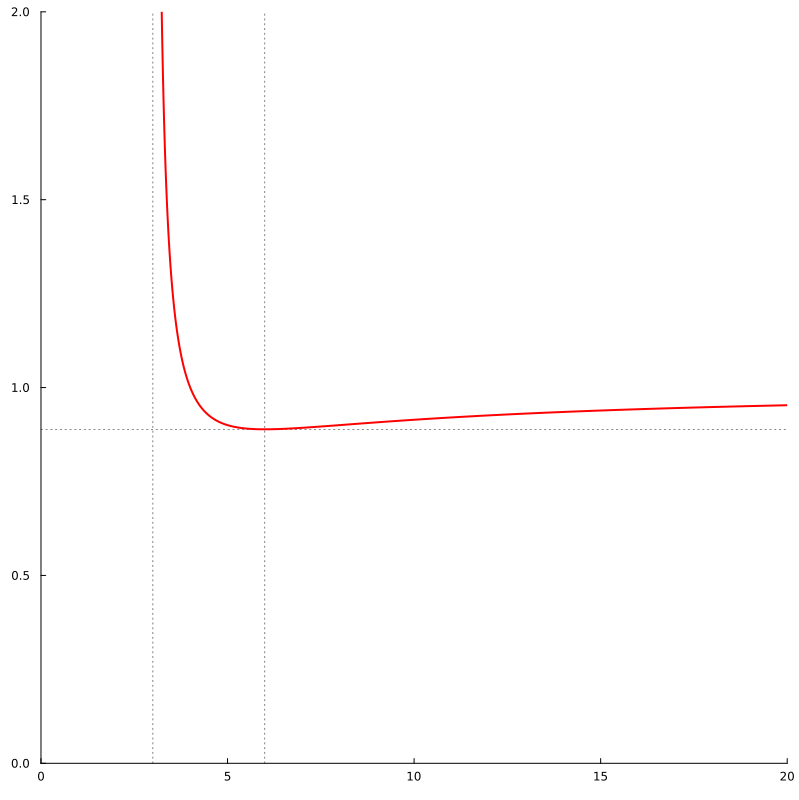
\includegraphics[width=0.5\columnwidth]{./images/schwarzschild/09.png}
    \caption{$E^2 - \left( \frac{r}{M} \right)$}
    \label{}
\end{figure}
\subsection{
	角運動量
}
$(6.2)$式より、
\[
\left( \frac{l}{M} \right)^2 = \frac{\left( \frac{r}{M} \right)^2}{ \left( \frac{r}{M} \right) - 3 }
\]
\[
\left( \frac{\partial \left( \frac{l}{M} \right) }{\partial \left( \frac{r}{M} \right)} \right)^2 = \frac{r}{M} \frac{ \left( \frac{r}{M} - 6 \right)}{ \left( \frac{r}{M} - 3 \right)^2 }
\]
\begin{figure}[H]
    \centering
    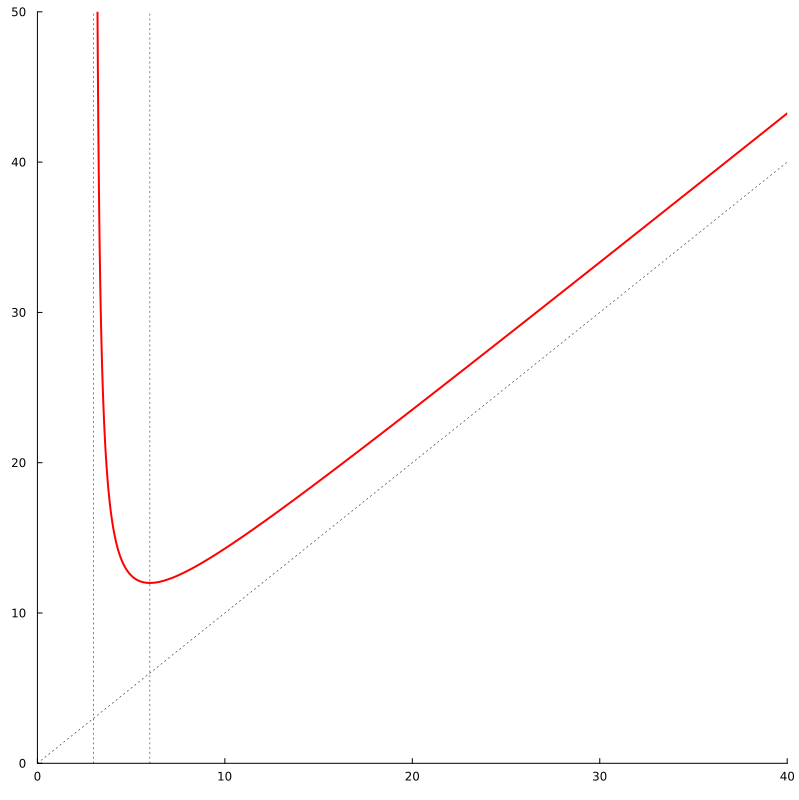
\includegraphics[width=0.5\columnwidth]{./images/schwarzschild/08.png}
    \caption{$\left( \frac{l}{M} \right)^2 - \left( \frac{r}{M} \right)$}
    \label{}
\end{figure}
\section{
	円軌道の安定性
}
\[
\frac{l}{M} \geq \sqrt{12}
\]
では、2点の$r$で円軌道をとることができる。\\
この2点$r_{-}, r_{+}$とすると、解析により
\begin{equation}
\begin{split}
3 < \frac{r_{-}}{M} \leq 6 \leq \frac{r_{+}}{M}
\end{split}
\end{equation}
がわかっていた。\\
\[
V(r) = - \frac{2M}{r^3} l^2 + \frac{l^2}{r^2} - \frac{2M}{r} + 1
\]
とすると
\[
\dot{r}^2 = E^2 - V(r)
\]
より
\begin{equation*}
\begin{split}
	\frac{d}{d \lambda} \dot{r}^2 &= \frac{d}{d\lambda} \left( E^2 - V(r) \right)\\
	2 \ddot{r} \dot{r} &= - \dot{r} V'(r)\\
	\ddot{r} &= - \frac{1}{2}V'(r)
\end{split}
\end{equation*}
円軌道に摂動$\delta r$が加わった際の、動径方向加わる力と加速度を考えると
\begin{equation*}
\begin{split}
	\ddot{r} + \delta \ddot{r} &= - \frac{1}{2} V'(r + \delta r)\\
	&= - \frac{1}{2} V'(r) - \frac{1}{2} V''(r)\delta r - ...
\end{split}
\end{equation*}
よって
\begin{tcolorbox}[title=摂動における微分方程式]
\begin{equation}
\begin{split}
	\delta \ddot{r} = - \frac{1}{2} V''(r)\delta r
\end{split}
\end{equation}
\end{tcolorbox}\noindent
この微分方程式を解くと
\begin{equation}
\begin{split}
	\delta r = C_1 \exp \left( \lambda \sqrt{-\frac{V''(r)}{2}} \right) + C_2 \exp \left( - \lambda \sqrt{-\frac{V''(r)}{2}} \right)
\end{split}
\end{equation}
そこで、$V''(r)$について考えると
\begin{equation}
\begin{split}
	V''(r) &= -\frac{24M}{r^5}l^2 + \frac{6}{r^4}l^2 - \frac{4M}{r^3}\\
	&= - \frac{12M}{r^5}l^2 + \frac{2}{r^4}l^2 -\frac{2}{r} \left( \frac{6M}{r^4} - \frac{2}{r^3}l^2 + \frac{2M}{r^2} \right)\\
	&= - \frac{12M}{r^5}l^2 + \frac{2}{r^4}l^2 -\frac{2}{r} V'(r)\\
	&= - \frac{12M}{r^5}l^2 + \frac{2}{r^4}l^2\\
	&= - \frac{2l^2}{r^4} \left( 6 \frac{M}{r} - 1 \right)\\
\end{split}
\end{equation}
$(6.3)$より\\
$r_{-}$の円軌道では$V''(r) \leq 0$なので\\
\[
	-\frac{V''(r)}{2} = a^2 \geq 0
\]
と置くと
\begin{equation*}
\begin{split}
	\delta r = C_1 \exp \left( \lambda a \right) + C_2 \exp \left( - \lambda a \right)
\end{split}
\end{equation*}
この値は$\lambda$とともに大きくなるので\\
$r_{-}$の軌道は不安定である。\\
$r_{+}$の円軌道では$0 \leq V''(r)$なので\\
\[
	\frac{V''(r)}{2} = a^2 \geq 0
\]
と置くと
\begin{equation*}
\begin{split}
	\delta r &= C_1 \exp \left( i \lambda a \right) + C_2 \exp \left( - i \lambda a \right)\\
	&= (C_1 + C_2)\cos (\lambda a) + i (C_1 - C_2)\sin (\lambda a)
\end{split}
\end{equation*}
この値は$\lambda$によって周期的に変化するが、$r$の大きさは発散しないので\\
$r_{+}$の起動は安定である。\\
\chapter{2024 06/26}
% =================================
% chapter 8
% =================================
\section{
	アインシュタインテンソル
}

\begin{equation*}
\begin{split}
	V(r) = \frac{Gm_1m_2}{r}
\end{split}
\end{equation*}

\section{
	シュワルツシルト時空における光の軌道
}

\section{
	ニュートン力学と相対論における二体問題の比較
}

\end{document}